\documentclass{article}

% if you need to pass options to natbib, use, e.g.:
%     \PassOptionsToPackage{numbers, compress}{natbib}
% before loading neurips_2018

% ready for submission
% \usepackage{neurips_2018}

% to compile a preprint version, e.g., for submission to arXiv, add add the
% [preprint] option:
%     \usepackage[preprint]{neurips_2018}

% to compile a camera-ready version, add the [final] option, e.g.:
     \usepackage[final]{neurips_2018}

% to avoid loading the natbib package, add option nonatbib:
\usepackage[nonatbib]{neurips_2018}

\usepackage[utf8]{inputenc} % allow utf-8 input
\usepackage[T1]{fontenc}    % use 8-bit T1 fonts
\usepackage{hyperref}       % hyperlinks
\usepackage{url}            % simple URL typesetting
\usepackage{booktabs}       % professional-quality tables
\usepackage{amsfonts}       % blackboard math symbols
\usepackage{nicefrac}       % compact symbols for 1/2, etc.
\usepackage{microtype}      % microtypography
\usepackage{graphicx}

\title{A data-driven study of cystic fibrosis treatment: identifying sub-types of physiotherapy style and physical activity using unsupervised clustering}

% The \author macro works with any number of authors. There are two commands
% used to separate the names and addresses of multiple authors: \And and \AND.
%
% Using \And between authors leaves it to LaTeX to determine where to break the
% lines. Using \AND forces a line break at that point. So, if LaTeX puts 3 of 4
% authors names on the first line, and the last on the second line, try using
% \AND instead of \And before the third author name.

%\author{%
%  David S.~Hippocampus\thanks{Use footnote for providing further information
%    about author (webpage, alternative address)---\emph{not} for acknowledging
%    funding agencies.} \\
%    I think we need to keep anonymous for our submission\\
%  Department of Computer Science\\
%  Cranberry-Lemon University\\
%  Pittsburgh, PA 15213 \\
%  \texttt{hippo@cs.cranberry-lemon.edu} \\
  % examples of more authors
  % \And
  % Coauthor \\
  % Affiliation \\
  % Address \\
  % \texttt{email} \\
  % \AND
  % Coauthor \\
  % Affiliation \\
  % Address \\
  % \texttt{email} \\
  % \And
  % Coauthor \\
  % Affiliation \\
  % Address \\
  % \texttt{email} \\
  % \And
  % Coauthor \\
  % Affiliation \\
  % Address \\
  % \texttt{email} \\
%}

\begin{document}


\maketitle

\begin{abstract}
  Children and young people with cystic fibrosis (CYPwCF) are prescribed physiotherapy including daily airway clearance techniques (ACT), and physical activity as part of their treatment. Little is known about how CYPwCF follow this advice in their everyday lives. Physiotherapy has evolved over the decades without this detailed data. Such data is now being collected as part of Project [anonymous] which is the largest CF physiotherapy trial in the UK to date. The data comes from novel pressure sensors attached to existing ACT devices which remotely measure breathing patterns during normal treatments, and Fitbit activity trackers which monitor physical activity patterns. In close collaboration with clinical experts, we quantify and characterise this unique ACT and activity data by creating custom features from the waveforms. Using unsupervised learning techniques, We identify meaningful sub-types, with k-means clustering achieving the best performance. We find 4 clusters of ACT data which are sensitive enough to track interventions in ACT routine. As pertaining to physical activity we identify 4 clusters of steps data and 5 clusters of heartrate data.
\end{abstract}

\section{Problem overview}

Cystic Fibrosis (CF) is a chronic life limiting illness affecting approximately 1 in 2500 babies born in the UK. CF is a systemic genetic disorder that mainly affects the respiratory and digestive systems. In the lungs excessive thick sticky mucus causes to a cycle of infection, inflammation and lung damage leading to a deterioration in health. Despite recent progress CF remains progressive and incurable. In some cases, a lung-transplant is performed, but only half of the current CF population are expected to live to over 40 years old [*******UCL****** ref to this or similar].  

To promote clearance of mucus from the lungs, daily physiotherapy including airway clearance techniques (ACT) are prescribed. The physiotherapy exercises involve a series of  exhalations against resistance into a handheld device  followed by a huff and cough to improve mucociliary clearance and expel mucous; an exercise which is performed repeatedly \cite{Villanuevaj4574} [*******UCL****** ref to guideline?]. For children with CF, the physiotherapy is burdensome, with some reporting that they dislike their physiotherapy more than they dislike the disease itself [*******UCL****** ref? This was from a survey that Jackie mentioned]. Physiotherapists also encourage children to have a physically active lifestyle, this has been shown to reduce the rate of decline in lung function [*******UCL****** ref to why physical activity is good]. Until recently adherence to physiotherapy recommendations was only assessed via questionnaire or self report which is known to be inaccurate with more objective methods not widely available [*******UCL****** ref]. The evolution of CF physiotherapy has not been informed by this important evidence.  

Bespoke pressure sensors were developed to attach to existing ACT devices and remotely monitor ACT breathing patterns. One way to reduce the treatment burden of ACT may be by using gamification. To investigate if gamification can change ACT adherence or patterns, bespoke games were developed which are driven by pressure changes measured with the sensor [ref 1: verbal description of games, ref 2: video demonstrating the point https://customers.microsoft.com/en-us/story/731791-fizzyo, removing any identifyin names in the bibliography]. Physical activity patterns were also measured using Fitbit activity trackers. 

 145 CYPwCF participated in the study [NREC:18-LO-1038] to quantify routine ACT (using bespoke pressure sensors) and physical activity patterns (via wearing of a Fitbit activity tracker), and to study the effects of gamification. This is the largest CF physiotherapy trial in the UK [*******UCL****** ref to meta-analysis of CF trials, or previously largest studies, or any previous data-driven studies?], collecting completely novel daily data about how children follow physiotherapy advice in their everyday lives. The broader goals of the study are to link physiotherapy behaviour patterns with clinical outcomes, in order to optimise and personalise treatment. In this paper we describe the challenge of i) quantifying ACT pressure sensor data and Fitbit activity data by creating custom features of the waveforms, and ii) discovering sub-types of ACTs and activity using clustering techniques. These daily sub-types can be tracked over time, as interventions such as gaming are introduced.   
\section{Methods}
\subsection{Trial design and analysis approach}
We used an interrupted time series design for the 18 month trial, so the effect on ACT patterns of introducing and removing an intervention can be assessed [[*******UCL****** ref to details of trial design,is this sufficient? NREC:18-LO-1038 ]. Interventions include introducing feedback to participants on their ACT (number of breaths) on a tablet application, introducing games, and later removing these interventions. The data presented here is from the first 8x months of the trial. Participants are: [*******UCL****** exact numbers] 65x males and 80x females ranging in age from 6-16 years old, from 3 London hospitals, and are voluntarily part of the study. All data is completely de-identified for analysis to researchers. 
 
Our analysis seeks to find patterns in physiotherapy data. Once these patterns are known, they can be linked with clinical outcomes to determine if certain behaviour patterns are preferable. We do not impose pre-conceived labels such as “good” or “bad” on waveforms, thus we leave open the possibility that what is currently prescribed may not be optimal. As such, the data is unlabelled and we use unsupervised learning approach to achieve this. Unsupervised clustering has been used to find sub-types in physical activity data \cite{physical_activity_patterns_2017} and pressure data relating to respiratory disease []. 

A high-scale data analysis and exploration pipeline was built in R in a secure analysis environment.  

\subsection{Collaboration, trust and interpretability}
Many applications of machine learning to medical data fail to explain how (if at all) the expertise of clinicians has been included \cite{Alaa2018}. To address the issues that arise from a lack of collaboration \cite{Vayena2018}, \cite{Challen231}, \cite{Char2018}, \cite{Ahmad2018} our methodology involves close collaboration between data scientists and CF experts, making every data decision jointly. We use a novel approach of involving at least one clinical expert in engineering “stand-ups” every day over the course of building the data analysis pipeline (7 months). We only consider features that are meaningful to clinicians, and we balance traditional statistical evaluation metrics, with what is interpretable to clinicians.  

\subsection{Feature engineering}
\subsubsection{Breath data description}
An ACT treatment commonly involves around 10 sets of 10 exhalation breaths into the ACT device. Each set loosens mucous, so that after the set the participant can huff and cough to expel it. The treatment may be performed once or twice per day; participants do not have identical prescriptions. The ACT device is fitted with a wireless pressure sensor sampling at 10 Hz, recording a pressure value (cm H2O) and its time stamp. Participants each used 1-3 of 4 different ACT devices compatible with the sensor; the Acapella, Aerobia, PariPEP and AstraPEP.  
\subsubsection{Processing breath data}
Several pre-processing steps were performed on the data which were a function of the custom sensor used: including assembling data packets and removing duplicate values. The sensor also introduced significant non-linear baseline drift. Because of the asymmetrical nature of the exhalation peaks and sparsity of the signal, we used a sparsity-based de-noising approach with an asymmetry factor, called BEADS \cite{Ning2014}, which is designed for use with chromatogram waveforms which have a similar form. 
% figure 1
In total, we recorded 5x,000 sensor readings. This includes data from every time the ACT sensor was turned on, including for testing and demonstration. Once we removed readings shorter than 15 seconds, treatments with no breath exhalations, and situations with sensor misuse/malfunction, we were left with 2x,000 ACT treatments for analysis. 

\subsubsection{Featurising breath data}
% figure 2
The defining characteristics of ACT treatments were summarised in a range of features (variables): breath count, breath duration, breath amplitude, and treatment duration. In order to derive these features, our breath identification algorithm recognises breaths composed of multiple peaks, and having breath shapes which are characteristic of the 3 different ACT devices used in the study. In addition to mean breath amplitude, we use amplitude standard deviation as a feature, in order to capture inconsistency or disorderliness in physiotherapy. We also identified how many discernible sets were apparent in the treatment. These features are on a per-treatment level. 

The aforementioned features capture the characteristics of existing treatments. However it is common for prescribed treatments to be skipped, and days with no treatments is an important signal itself. Several features were derived which capture missing data: treatment adherence to date, skipped days since last treatment, rolling adherence over 7 days. These features are on a per-day level, as participants are prescribed 1 or 2 treatments per day. 


\subsubsection{Featurising physical activity data}
The Fitbit activity tracker (Fitbit AltaHR) provides each participant’s step count per minute. While real-time heartbeat data would allow for a detailed analysis of heartrate waveforms, the Fitbit only provides average heartrate, with a variable sampling frequency ranging from 3 to 12 values per minute. To achieve consistent frequency and comparable values, the heartrate values are averaged for each minute.   

Mindful of these data limitations, we extract high-level patterns from the minute averaged waveforms at a day level. The heartrate and steps datasets are featurised using summary statistics per day using counts, frequency and interval values such as number of minutes in moderate to vigorous intensity physical activities (MVPA) (heartrate above 120 bpm) per day, step cadence (number of steps/minutes of wear) at day level, and number of hours with more than 500 steps at day level. 

% figure 3

\subsubsection{Missing activity data}

To account for missing data during times that the Fitbit is not worn, the wear percent of the Fitbit is calculated from the heartrate values. This measure is used to select only days with a substantial portion of data for the day (80\% of wear time from 6 am to 6 pm) for analysis. The wear time is also used to normalise some features and to obtain step cadence for minutes where heartrate data is present. 

\subsubsection{Clustering to find sub-types}  

All features were verified by clinicians as being meaningful or potentially meaningful. We perform a correlation analysis on all features and removed features which were highly correlated. We use the Hopkins statistic [ref] to measure clustering tendency. Features with a Gaussian distribution are normalised to have mean =0 and standard deviation 1. In order to visualise the results, we use dimensionality reduction. We use the first two principle components from principal component analysis [ref], Uniform Manifold Approximation and Projection (UMAP), and t-Distributed Stochastic Neighbor Embedding (T-SNE). We identify outliers using xxx methods and remove less than 2\%, with these cases being recognised as device malfunctions or unusual human behaviour.  

We employ the following clustering methods: k-means, Density-based spatial clustering of applications with noise (DBSCAN) and hierarchical clustering.  

\section{Results}
\subsection{Clustering breath waveforms}
\subsubsection{Feature selection for clustering}
Some features were excluded from clustering, but provide interesting physiotherapy insights.  
The number of sets in a treatment were expected to be very influential in clustering, as a regular pattern of sets shows close adherence to physiotherapy advice. However we found that less than 20xx\% of treatments had discernible sets, so this feature could not be used

% table 1

\subsubsection{ACT clustering results}
The results of the four techniques used for clustering are show in table x. K-means was found to perform best because we liked the way..… K-means is a simple 

% table 2
% table 3
% figure 4

\subsubsection{ACT clustering validation}

We have checked the clustering stability on different data partitions.  Random sampling of the data (80\% of data) and using k-means clustering provided very similar results comparing to clustering on the full dataset:  shape of the clusters, cluster centroids as well as Silhouette Coefficients and Calinski-Harabaz Index  (2200 v 1770 respectively) are comparable. 
% figure
We also have done validation of the clusters by adding or removing features and checking individual patients’ representation and trajectory in those clusters. Figure xx shows the same patient trajectory for the Clustering A and Clustering B. Clustering B uses breath amplitude features (mean and standard dev) as well as breathRollWeekAdherenceScore in addition to features that Clustering A uses. Notable that  once computer gaming is introduced to ACT in both cases A and B the same patient moves from cluster with “expected” breath counts per ACT to cluster characterized by much bigger breath counts. This validates that there is a change in patient’s behaviour that we’ve captured. Additional sdBreathAmplitude feature make results more explainable from clinical point of view as original cluster for the patient in Clustering B was characterized by centroid with the biggest sdBreathAmplitude value. 
% figure

\subsection{Clustering physical activity waveforms} 

Clustering of physical activity data was used to extract daily patterns from the steps and heartrate waveforms that can be utilised to individually characterise the physical activity levels and patterns of individual patients. The different clusters should extract more complex characteristics than the ones which could be obtained by simply combining some of the extracted features. 

\subsubsection{Steps clusters}

The following features were used for clustering steps: number of minutes with step count higher than 100 for at least 5 consecutive minutes, the mean of total step count per hour, the step cadence for the periods in MVPA and the number of hours in the day with 0 < steps count < 500. Features were selected as a result of feature selection, correlation and outlier analysis. Four clusters were found by Kmeans with the following characteristics: 

\begin{itemize}
\item XS - this cluster contains waveforms with very little steps activity or much missing step data 
\item S - moderate step activity and consistent cadence throughout the day with very few periods of high step activity 
\item M - consistent moderate to high step rate across the day with period of sustained high step activity  
\item L - High step rate throughout the day with longer periods of sustained high step activity
\end{itemize}
%figure
%table

subsubsection{Heartrate clusters}

The number of minutes with heartrate higher than 120, coefficient of variation for heartrate values at a day level, number of time heartrate goes above 100 and 120 and the median average hourly heartrate were used as features for the heartrate clusters. Five clusters were found by Kmeans with the following chacteristics: 
\begin{itemize}
\item S - Small heartrate values and consistently below 120 
\item M - Consistent variations around 100 with very few spikes in heartrate values 
\item M1 - Waveform with high variability and periods with spikes above 120 and fluctuations above the 120 mark 
\item M2 - Consistent variations around 100 with spikes in values above 120 
\item L - Large values around and above 120 
\end{itemize}
%figure
%table


\subsubsection{Fitbit cluster validation }

The steps and heartrate clusters were validated with the clinical experts. Individual waveforms were manually inspected together with the cluster boundaries to ensure consistency across cluster interpretations and the actual cluster characteristics. Additionally, other features that were not included in the clustering analysis were used to validate the clusters and their interpretations. Certain expected conditions were checked against the cluster labels and plotted using the PCA graph such as Figure Xxx below. 


\section{Discussion and conclusion} 

Project Fizzyo involves collecting novel data about how CF physiotherapy advice, ACTs and physical activity, is adhered to. In close collaboration with CF experts, we develop methods to interrogate this data. We derive clinically meaningful features from ACT and activity (heartrate and steps) waveforms. We use unsupervised clustering to find sub-types of this data. 

Project Fizzyo is an ongoing study, with participation lasting 18 months. 7 months into the trial we do not draw any conclusions, as we do not have an equal number of days of data from patients. Instead, we present a framework for analysis, which will empower clinicians to interpret the impact of interventions such as gamification, and what type of physiotherapy leads to better clinical outcomes.

\section{Usage of tables and figures}
\subsection{Figures}

\begin{figure}
  \centering
  \caption{Sample figure caption.}
  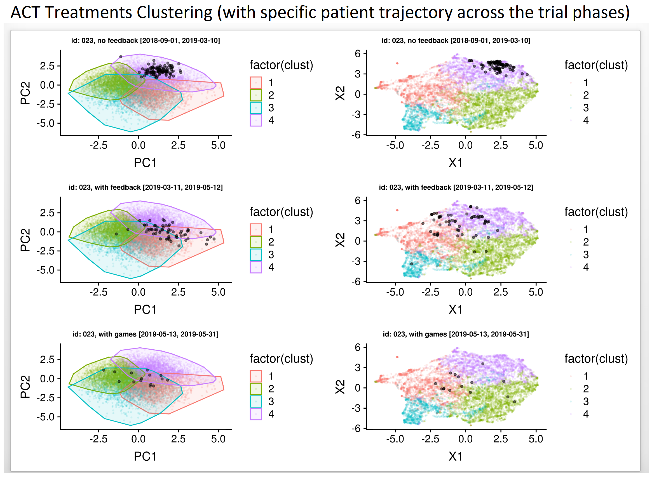
\includegraphics[]{sample_fig}
\end{figure}

\subsection{Tables}
\begin{table}
  \caption{Sample table title}
  \label{sample_table}
  \centering
  \begin{tabular}{lll}
    \toprule
    \cmidrule(r){1-2}
    Col1 & Col2 & Col3 \\
    \midrule
    a & 0 & z\\
    b & 1 & y \\
    c & 2 & x \\
    \bottomrule
  \end{tabular}
\end{table}

Here is how you can reference a table \ref{sample_table}

\bibliographystyle{abbrv}
% include your .bib file
\bibliography{fizzyo}

\appendix
\section{Appendix : Table of physical activity data features}

\begin{table}[h]
  \caption{Physical activity features}
  \label{fitbit_features}
  \centering
  \begin{tabular}{ |l|l|l| }
    \toprule
    \cmidrule(r){1-2}
    \textbf{Feature Name} & \textbf{Feature description} & \textbf{Waveform extracted from} \\
    \midrule
    Active Hours & Number of hours with a step count > 500 & Steps waveform \\
    \bottomrule
    \end{tabular}
\end{table}

\appendix
\section{Appendix : Table of ACT treatment features}

\begin{table}[h]
  \caption{ACT features}
  \label{act_features}
  \centering
  \begin{tabular}{ |l|l| }
    \toprule
    \cmidrule(r){1-2}
    \textbf{Feature Name} & \textbf{Feature description} \\
    \midrule
    Breath Count & Number of breaths the person has made though an ACT  \\ 
     ~ & device during a treatment. A breath is counted if its maximum amplitude is \\ ~ & above the threshold of 8 mm H2O.\\
     \midrule
     Mean Breath Amplitude & Average breath amplitude (in mm H2O) during an ACT treatment. \\
     Minimum Breath Amplitude & Similarly minimum, maximum and standard deviation of breath amplitude. \\
     Maximum Breath Amplitude & ~ \\
     Standard Deviation of Breath Amplitude & ~\\
     \midrule
     Mean Breath Duration & Average duration (in seconds) of breath during an ACT treatment.\\ 
     Minimum Breath Duration &  Similarly minimum, maximum and standard deviation of \\ 
     Maximum Break Duration & breath duration in a treatment. \\
     Standard Deviation of Breath Duration & ~\\
     \midrule
     Break Count & Number of breaks (between breaths) in a treatment. \\
     \midrule
     Mean Break Duration & Average duration (in seconds) of breaks between breaths.\\ 
     Minimum Break Duration & Similarly minimum, maximum and standard deviation of \\ 
     Maximum Break Duration & breaks duration in a treatment. \\
     Standard Deviation of Break Duration & ~\\
     \midrule
     Set Count & Number of sets in a treatment. Prescribed treatment may have up to 10 \\
     ~ & sets. Set is a group of breaths separated by huffing and coughing activity.\\
     \midrule
     Pressure Readings Count & Number of pressure reading registered by ACT device during a treatment. \\
     ~ & Used to filter out "test" device sessions that are not part of a treatment.\\
     \midrule
     Pressures Readings Completeness Score & Data completeness score for the day \\
     ~ & If a treatment has less than 150 pressure readings it's completeness \\
     ~ & score is 0. \\
     \midrule
     Treatment Duration & Treatment duration (in minutes).\\
     \midrule
     Treatment Daily Adherence Score & Number of completed treatments out of the prescribed ones (for the \\
     ~ & given day). \\
     \midrule
     Breath Count Daily Adherence Score & Number of registered breaths across all treatments for the given day \\
     ~ & out of the prescribed amount of breaths. \\ 
     \midrule
     Treatment Rolling Weekly Adherence Score & Number of completed treatments during the last 7 days (for a given date) \\
     ~ & out of the prescribed number of treatments for this period. \\
     \midrule
     Breath Count Rolling Weekly Adherence Score & Number of registered breaths across all treatments during the last 7 days\\
     ~ & (for a given date) out of the prescribed amount of breaths for this period.\ 
     \midrule
     Treatment Weekly Adherence Score & Number of completed treatments during the last calendar week (for a given date) \\
     ~ & out of the prescribed number of treatments for this period. \\
     \midrule
     Breath Count Weekly Adherence Score & Number of registered breaths across all treatments during the last calendar week \\
     ~ & (for a given date) out of the prescribed amount of breaths for this period.\\
     \midrule
     Cumulative Adherence Score & Cumulative adherence score to date. \\
     ~ & How many in total treatments patient done over a period (since the beginning of the study out the prescribed amount.\\
     \midrule
     Breathing Time Percentage & Time in a treatment spent on an exhalation, vs not.\\
     \midrule
     Skipped Days Count & Skipped days since the last treatment. \\
     \bottomrule
    \end{tabular}
\end{table}

\section{Appendix : Cluster metrics for physical activity data}

The tables below show the metrics for the clusters identified for the physical activity data. 

\textbf{Steps clusters}

Calinski-harabasz index for the steps clusters is 6021.14 .

\begin{table}[h]
  \caption{Steps clusters Metrics}
  \label{steps_metrics}
  \centering
  \begin{tabular}{ |l|c|c|}
    \toprule
    \cmidrule(r){1-2}
    Cluster name & Cluster Size & Average Silhouette width \\
    \midrule
    XS & 1099 & 0.95 \\
    S & 3942 & 0.34 \\
    M & 2737 & 0.27 \\
    L & 1982 & 0.24 \\
    \bottomrule
    \end{tabular}
\end{table}

\textbf{Heartrate clusters}

Calinski-harabasz index for the heartrate clusters is 5090.37 .

\begin{table}[h]
  \caption{Heartrate clusters Metrics}
  \label{hr_metrics}
  \centering
  \begin{tabular}{ |l|c|c|}
    \toprule
    \cmidrule(r){1-2}
    Cluster name & Cluster Size & Average Silhouette width \\
    \midrule
    S & 1246 & 0.28 \\
    SM & 1640 & 0.2 \\
    M1 & 2308 & 0.21 \\
    M2 & 2584 & 0.26 \\
    L & 1982 & 0.33 \\
    \bottomrule
    \end{tabular}
\end{table}

\end{document}